%% Template originaly created by Karol Kozioł (mail@karol-koziol.net) and modified for ShareLaTeX use

\documentclass[a4paper,11pt]{article}

\usepackage[T1]{fontenc}
\usepackage[utf8]{inputenc}
\usepackage{graphicx}
\usepackage{xcolor}
\renewcommand\familydefault{\rmdefault}
\usepackage{tgheros}

\usepackage{amsmath,amssymb,amsthm,textcomp}
\usepackage{enumerate}
\usepackage{multicol}
\usepackage{tikz}
\usepackage[utf8]{vietnam}
\usepackage[unicode]{hyperref}
\usepackage{mathtools}

\newcommand\Myperm[2][^n]{\prescript{#1\mkern-2.5mu}{}P_{#2}}
\newcommand\Mycomb[2][^n]{\prescript{#1\mkern-0.5mu}{}C_{#2}}
\usepackage{geometry}
\geometry{total={210mm,297mm},
left=25mm,right=25mm,%
bindingoffset=0mm, top=22mm,bottom=25mm}

\linespread{1.3}

\newcommand{\linia}{\rule{\linewidth}{0.5pt}}

% custom theorems if needed
\newtheoremstyle{mytheor}
    {1ex}{1ex}{\normalfont}{0pt}{\scshape}{.}{1ex}
    {{\thmname{#1 }}{\thmnumber{#2}}{\thmnote{ (#3)}}}

\theoremstyle{mytheor}
\newtheorem{defi}{Definition}

% my own titles
\makeatletter
\renewcommand{\maketitle}{
\begin{center}
\vspace{2ex}
{\huge \textsc{\@title}}
\vspace{1ex}
\\
\linia\\
\@author \hfill \@date
\vspace{4ex}
\end{center}
}
\makeatother
%%%

% custom footers and headers
\usepackage{fancyhdr}
\setlength{\headheight}{20pt}
\pagestyle{fancy}
\fancyhead{} % clear all header fields
\fancyhead[L]{
 \begin{tabular}{rl}
    \begin{picture}(15,10)(0,0)
    \put(0,-8){
\includegraphics[width=8mm, height=8mm]{hcmut.png}}
    %\put(0,-8){\epsfig{width=10mm,figure=hcmut.eps}}
   \end{picture}&
	%
\includegraphics[width=8mm, height=8mm]{hcmut.png} & %
	\begin{tabular}{l}
		\textbf{\bf \ttfamily Ho Chi Minh City, University of Technology}\\
		\textbf{\bf \ttfamily Department of Computer Science and Engineer}
	\end{tabular} 	
 \end{tabular}
}
\fancyhead[R]{
	\begin{tabular}{l}
		\tiny \bf \\
		\tiny \bf 
	\end{tabular}  }
\fancyfoot{} % clear all footer fields
\fancyfoot[L]{\scriptsize \ttfamily Nghiên cứu phát triển kỹ thuật đếm số phần tử trên dòng dữ liệu}
\rfoot{Trang \thepage}
\renewcommand{\headrulewidth}{0.2pt}
\renewcommand{\footrulewidth}{0.2pt}
%



% code listing settings
\usepackage{listings}
\lstset{
    language=Python,
    basicstyle=\ttfamily\small,
    aboveskip={1.0\baselineskip},
    belowskip={1.0\baselineskip},
    columns=fixed,
    extendedchars=true,
    breaklines=true,
    tabsize=4,
    prebreak=\raisebox{0ex}[0ex][0ex]{\ensuremath{\hookleftarrow}},
    frame=lines,
    showtabs=false,
    showspaces=false,
    showstringspaces=false,
    keywordstyle=\color[rgb]{0.627,0.126,0.941},
    commentstyle=\color[rgb]{0.133,0.545,0.133},
    stringstyle=\color[rgb]{01,0,0},
    numbers=left,
    numberstyle=\small,
    stepnumber=1,
    numbersep=10pt,
    captionpos=t,
    escapeinside={\%*}{*)}
}

%%%----------%%%----------%%%----------%%%----------%%%

\begin{document}

\begin{titlepage}
\begin{center} {\textbf{ĐẠI HỌC QUỐC GIA TP. HỒ CHÍ MINH}
}

{\textbf{TRƯỜNG ĐẠI HỌC BÁCH KHOA}
}

{\textbf{KHOA KHOA HỌC VÀ KỸ THUẬT MÁY TÍNH }
}

{\textbf{---------------------------------------}}

\end{center}

\vspace{1cm}

\begin{figure}[h!]
\begin{center}

\includegraphics[width=3cm]{hcmut.png}
\end{center}
\end{figure}

\vspace{2cm}


\begin{center}
\begin{tabular}{c}
%\multicolumn{1}{c}{\textbf{{\Large BÁO CÁO BÀI TẬP LỚN}}}
\multicolumn{1}{c}{\textbf{\Large NGHIÊN CỨU PHÁT TRIỂN KỸ THUẬT ĐẾM SỐ PHẦN TỬ TRÊN DÒNG DỮ LIỆU}}
\vspace{2cm}
\\
\multicolumn{1}{c}{\textbf{\Large LUẬN VĂN THẠC SĨ}}


~~\\

\\
\multicolumn{1}{l}{\textbf{{\Large}}}\\
\\
\textbf{{\Large}}\\

\\
\\

\end{tabular}
\end{center}

\vspace{1cm}

\begin{table}[h]
\begin{tabular}{rrl}
\hspace{5.1cm} 
&\textit{Học viên: } & \textbf{LÊ ANH QUỐC}\\
&\textit{ID: } & \textbf{2070428}\\

\end{tabular}
\end{table}
\vspace{3cm}
\begin{center}
{\footnotesize HỒ CHÍ MINH CITY}
\end{center}
\end{titlepage}
%%%----------%%%----------%%%----------%%%----------%%%
%\begin{document}

\begin{titlepage}
\begin{center} {\textbf{ĐẠI HỌC QUỐC GIA TP. HỒ CHÍ MINH}
}

{\textbf{TRƯỜNG ĐẠI HỌC BÁCH KHOA}
}

{\textbf{KHOA KHOA HỌC VÀ KỸ THUẬT MÁY TÍNH }
}

{\textbf{---------------------------------------}}

\end{center}

\vspace{1cm}

\begin{figure}[h!]
\begin{center}

\includegraphics[width=3cm]{hcmut.png}
\end{center}
\end{figure}

\vspace{2cm}


\begin{center}
\begin{tabular}{c}
%\multicolumn{1}{c}{\textbf{{\Large BÁO CÁO BÀI TẬP LỚN}}}
\multicolumn{1}{c}{\textbf{\Large NGHIÊN CỨU PHÁT TRIỂN KỸ THUẬT ĐẾM SỐ PHẦN TỬ TRÊN DÒNG DỮ LIỆU}}
\vspace{2cm}
\\
\multicolumn{1}{c}{\textbf{\Large LUẬN VĂN THẠC SĨ}}

\vspace{0.5cm}
\\
\multicolumn{1}{c}{\text{\small NGÀNH: KHOA HỌC MÁY TÍNH }}
\vspace{0.5cm}
\\
\multicolumn{1}{c}{\text{\small MÃ NGÀNH: \textbf{8480101} }}
\vspace{1cm}
\\
\multicolumn{1}{c}{\textbf{\small NGƯỜI HƯỚNG DẪN KHOA HỌC }}
~~\\
\multicolumn{1}{c}{\textbf{\small PGS. TS. THOẠI NAM
 }}

\\
\\

\\
\\

\end{tabular}
\end{center}

\vspace{1cm}

\begin{table}[h]
\begin{tabular}{rrl}
\hspace{5.6cm} 
&\textit{Học viên: } & \textbf{lÊ ANH QUỐC}\\
&\textit{ID: } & \textbf{2070428}\\

\end{tabular}
\end{table}
\vspace{1cm}
\begin{center}
{\footnotesize HỒ CHÍ MINH CITY}
\end{center}
\end{titlepage}

%%%----------%%%----------%%%----------%%%----------%%%


%\thispagestyle{empty}

\renewcommand{\contentsname}{Content}
\newpage
\vspace{1cm}
\tableofcontents
\newpage
\section{GIỚI THIỆU ĐỀ TÀI, MỤC TIÊU VÀ ĐỐI TƯỢNG NGHIÊN CỨU}
\subsection{Tính cấp thiết và lý do chọn đề tài}
\hspace{2em}Ngày nay, các ứng dụng và dịch vụ trực tuyến đóng vai trò ngày càng quan trọng trong cuộc sống của con người. 
Chúng ta sử dụng mạng xã hội để kết nối với bạn bè và chia sẻ thông tin, mua sắm trực tuyến để tiết kiệm thời gian và tiền bạc, 
hay xem phim và chơi game trực tuyến để giải trí. Để đánh giá hiệu quả hoạt động của các ứng dụng và dịch vụ này, 
một trọng những chỉ số quan trọng nhất là số lượng người dùng hoạt động Distinct Active Users (DAU).

Việc theo dõi số lượng người dùng hoạt động trong một khoảng thời gian nhất định trên một dòng dữ liệu (data stream) 
là một yêu cầu quan trọng đối với nhiều ứng dụng và dịch vụ trực tuyến, hiệu quả của các chiến dịch marketing, 
và hỗ trợ ra quyết định kinh doanh. Ví dụ, trong các ứng dụng mạng xã hội, số lượng người dùng hoạt động cho thấy mức độ tương tác 
và sự quan tâm của người dùng đối với nền tảng. Trong các dịch vụ thương mại điện tử, số lượng người dùng hoạt động cho thấy hiệu quả 
và các chiến dịch quảng cáo và khuyến mãi. Tuy nhiên, việc đếm số lượng DAU không phải là một nhiệm vụ đơn giản, đặc biệt là khi dữ liệu lớn 
và tốc độ truy cập cao. Các phương pháp truyền thống như lưu trữ và truy vấn trực tiếp vào cơ sở dữ liệu có thể gặp nhiều hạn chế về hiệu suất 
và khả năng mở rộng.

Trong nhiều trường hợp, cần phải tổng hợp số lượng DAU trên nhiều streams hoặc services khác nhau. Việc này giúp có được bức tranh toàn cảnh về hoạt động của người dùng trên toàn hệ thống, từ đó đưa ra các phân tích và đánh giá chính xác hơn. Ví dụ, trong hệ thống thương mại điện tử, cần tổng hợp số lượng DAU từ các trang web, ứng dụng di động và API khác nhau để có được số lượng người dùng hoạt động thực tế trên toàn hệ thống. Tuy nhiên, việc tổng hợp dữ liệu từ nhiều nguồn khác nhau có thể gặp thách thức về đồng bộ hóa dữ liệu, xử lý dữ liệu bị thiếu hoặc lỗi, và đảm bảo tính nhất quán của kết quả. 

Ngoài ra, có thể cần phải đếm DAU trên nhiều đoạn khác nhau trong một stream, hoặc nhiều streams khác nhau. Việc này giúp phân tích chi tiết hơn hoạt động của người dùng theo thời gian, theo khu vực hoặc theo tiêu chí khác. Ví dụ, trong một ứng dụng phát trực tiếp, cần đếm số lượng người dùng hoạt động theo từng giờ hoặc từng phân đoạn chương trình để đánh giá mức độ quan tâm của người xem. Tuy nhiên, việc phân chia và xử lý dữ liệu theo nhiều đoạn có thể làm tăng độ phức tạp của thuật toán và ảnh hưởng đến hiệu suất của hệ thống. Do đó, cần phải có một giải pháp đếm số lượng phần tử trên dòng dữ liệu đạt hiệu suất cao và tin cậy, từ đó có thể ứng dụng rộng rãi trong các hệ thống khác nhau như mạng xã hội, thương mại điện tử, chương trình phát trực tiếp, hệ thống giám sát và hệ thống giao thông thông minh.

\subsection{Mục tiêu nghiên cứu }
\subsubsection{Phát triển thuật toán để đếm DAU trên một dòng dữ liệu (data stream):}
Thiết kế thuật toán sử dụng HyperLogLog để đếm DAU trên một khung thời gian trên một stream với độ chính xác cao và hiệu quả tốt. Ví dụ, đếm số lượng users đăng nhập vào hệ thống trong 5 phút trước, 1 giờ trước, 1 ngày trước hay 1 tháng trước.
\subsubsection{Mở rộng thuật toán để đếm DAU trong một khoảng thời gian trên nhiều streams:}
\subsubsection{Phát triển một thuật toán để đếm DAU trên nhiều khung thời gian và trên nhiều streams hoặc services khác nhau:}
Phát triển phương pháp và công cụ giám sát: Mục tiêu chính là thiết kế và phát triển các phương pháp và công cụ giám sát pin hiệu quả trên xe điện. Điều này bao gồm việc xác định các thông số quan trọng cần được giám sát như trạng thái sạc, nhiệt độ, dòng điện và điện áp của pin. Công cụ giám sát cần có khả năng thu thập, xử lý và hiển thị dữ liệu pin một cách dễ dàng và đáng tin cậy.\\
Phân tích và đánh giá hiệu suất hoạt động của pin: Mục tiêu là phân tích và đánh giá hiệu suất hoạt động của pin trên xe điện. Điều này có thể bao gồm việc theo dõi và ghi nhận các thông số pin trong quá trình vận hành, phân tích các dữ liệu thu thập được để đánh giá hiệu suất sạc, xả và tổn thất năng lượng. Mục tiêu cuối cùng là tối ưu hóa sử dụng năng lượng và kéo dài tuổi thọ pin thông qua các biện pháp quản lý phù hợp.\\
Phát hiện sớm các vấn đề và rủi ro: Mục tiêu là phát triển các thuật toán và phương pháp giám sát pin để phát hiện sớm các vấn đề và rủi ro tiềm ẩn. Điều này bao gồm việc xây dựng các mô hình dự đoán và cảnh báo để nhận biết các tình huống nguy hiểm như quá nhiệt, quá dòng, hao mòn pin nhanh chóng và các lỗi khác. Mục tiêu là nâng cao mức độ an toàn và độ tin cậy của hệ thống pin trên xe điện.\\
Nghiên cứu và ứng dụng công nghệ mới: Mục tiêu cuối cùng là nghiên cứu và áp dụng các công nghệ mới để cải thiện giám sát pin trên xe điện. Điều này có thể bao gồm việc sử dụng các cảm biến tiên tiến, hệ thống ghi dữ liệu thông minh, trí tuệ nhân tạo và học máy để tăng cường khả năng giám sát và dự đoán của hệ thống. Mục tiêu là tạo ra một hệ thống giám sát pin tiên tiến, đáng tin cậy và hiệu quả cho xe điện.

\subsection{Giới hạn và đối tượng nghiên cứu }
\subsubsection{Giới hạn}
Độ chính xác và độ tin cậy: Một trong những thách thức chính là đảm bảo độ chính xác và độ tin cậy của hệ thống giám sát pin trên xe điện. Các thông số pin cần được đo lường và giám sát một cách chính xác để đưa ra các quyết định đúng đắn và đảm bảo an toàn. Đồng thời, hệ thống giám sát phải đảm bảo tính tin cậy trong môi trường hoạt động khắc nghiệt và đảm bảo hoạt động liên tục của xe điện.\\
Quản lý dữ liệu: Việc giám sát pin trên xe điện có thể tạo ra lượng lớn dữ liệu, và việc quản lý và xử lý dữ liệu một cách hiệu quả là một thách thức. Cần phải xây dựng các phương pháp, công nghệ và hệ thống để thu thập, lưu trữ, xử lý và phân tích dữ liệu pin một cách hiệu quả và đáng tin cậy.
\subsubsection{Đối tượng nghiên cứu }
Đối tượng nghiên cứu của đề tài "Giám sát pin trên xe điện" là các yếu tố liên quan đến pin và hệ thống giám sát pin trên xe điện, nhằm tối ưu hóa hiệu suất, tuổi thọ và an toàn của pin trong hoạt động của xe điện.

\section{CÁC CÔNG TRÌNH NGHIÊN CỨU LIÊN QUAN }
- \textbf{Battery Management Systems in Electric and Hybrid Vehicles} – [1] Công trình này tập trung vào khái niệm và chức năng của hệ thống quản lý pin (BMS) trong xe điện và hybrid. Nó giới thiệu các yếu tố quan trọng trong việc giám sát pin như trạng thái sạc, nhiệt độ, điện áp và dòng điện, cũng như các chiến lược quản lý pin để tăng hiệu suất và tuổi thọ của pin.\\

- \textbf{State of Charge Estimation of Lithium-Ion Batteries in Electric Vehicles: A Review} – [2] Công trình này tập trung vào việc ước lượng trạng thái sạc của pin Lithium-Ion trong xe điện. Nó xem xét các phương pháp và thuật toán được sử dụng để ước lượng trạng thái sạc và đánh giá hiệu suất của chúng.\\

- \textbf{Real-Time State of Health Estimation for Lithium-Ion Batteries in Electric Vehicles} – [3] Công trình này tập trung vào ước lượng trạng thái sức khỏe (SOH) của pin Lithium-Ion trong xe điện. Nó đề xuất một phương pháp ước lượng SOH dựa trên phân tích dữ liệu pin thời gian thực và sử dụng mô hình dự đoán để đánh giá tuổi thọ còn lại của pin.\\

- \textbf{Data-Driven Fault Diagnosis and Prognosis of Lithium-Ion Batteries in Electric Vehicles} – [4] Công trình này tập trung vào việc chẩn đoán và tiên đoán lỗi cho pin Lithium-Ion trong xe điện. Nó sử dụng phương pháp dựa trên dữ liệu để phân tích và phát hiện các lỗi potentiostatic, impedance và voltage của pin, cung cấp thông tin quan trọng để dự đoán tuổi thọ và hiệu suất của pin.\\

- \textbf{Intelligent Battery Management and Control for Electric Vehicles} – [5] Công trình này tập trung vào nghiên cứu về quản lý và điều khiển pin thông minh cho xe điện. Nó đề xuất một hệ thống BMS thông minh sử dụng công nghệ trí tuệ nhân tạo và học máy để giám sát và dự đoán trạng thái pin, tối ưu hóa sử dụng năng lượng và quản lý tuổi thọ của pin.\\


\section{CÁC PHƯƠNG PHÁP TỐI ƯU }
Similar to the sensor, the implement of the gateway is presented in this part. However, instead of the whole source code (in java), some main parts are required to presented only.


\subsection{Trạng thái sạc (SOC)}
Tình trạng sạc (SoC - State of Charge) được coi là một trong những lĩnh vực nghiên cứu cốt lõi trong hệ thống quản lý năng lượng pin. Hầu hết các bài báo được chọn giới thiệu những phương pháp và tiếp cận mới để ước lượng SoC. Sai số trung bình bình phương là nhỏ hơn 3,146 và 2,315 cho các pin đã lão hóa và các loại pin khác nhau. Chiến lược cân bằng SoC dựa trên chia sẻ năng lượng dựa trên một kiến trúc BESS (Battery Energy Storage System) phân tán trong đó hệ thống cân bằng các ô pin và điều chỉnh điện áp DC bus được hợp nhất thành một hệ thống duy nhất. Các bộ chuyển đổi công suất nhỏ được sử dụng để cung cấp cân bằng SoC giữa các ô pin và quản lý điện áp DC bus. Các tác giả cho biết hiệu suất tổng thể của hệ thống hoàn chỉnh là 95-97. Dựa trên dòng điện và điện áp đo được, đã thiết kế một mô hình pin dựa trên mạng nơ-ron (ANN) để ước lượng SoC. Việc ước lượng SoC dựa trên mạng nơ-ron đã được cải thiện bằng cách sử dụng bộ lọc Kalman không mùi. Mô hình đề xuất được xác nhận bằng các chu kỳ lái xe EV (Electric Vehicle) trong các điều kiện nhiệt độ khác nhau. Một kỹ thuật SoC dựa trên mô hình điện hóa toàn diện của pin lithium-ion được trình bày bởi Klein. Các tác giả trình bày một bộ quan sát phạm vi lỗi đầu ra dựa trên một tập hợp giảm của phương trình đại số-giải phương trình vi phân. Các tác giả cho biết sai số SoC là nhỏ hơn 10.\\

SOC (State of Charge) còn là một yếu tố quan trọng nhưng không thể đo được dựa trên các công nghệ cảm biến hiện tại trên xe. Tỷ lệ giữa dung lượng hiện tại có sẵn và dung lượng tối đa có thể được biểu diễn dưới dạng SOC [11], được tính bằng Công thức (1):\\
\[SOC = 1 - \frac{\int(idt)}{Cn}\]

với i là dòng điện, còn Cn là dung lượng tối đa mà pin có thể chứa. \\

SOC (Trạng thái sạc) phản ánh lượng điện còn lại có sẵn cho pin. Nó được sử dụng để xác định quãng đường lái còn lại trong xe điện (EVs) và chỉ ra khi nào động cơ đốt trong xe hybrid (HEVs) nên được bật hoặc tắt [12]. Do các phản ứng hóa học tự nhiên trong pin và các tải trọng ngoại vi khác nhau, dung lượng tối đa của pin giảm dần theo thời gian. Sự không chắc chắn liên quan đến những yếu tố này sẽ dẫn đến đặc tính suy giảm của pin không tuyến tính, không ổn định. Phương pháp tiếp cận đơn giản nhất để ước lượng SOC là Coulomb counting (đếm Coulomb), phản ánh năng lượng trong pin dưới dạng Coulomb. Phương pháp này tính toán dung lượng pin bằng cách tích phân dòng điện vào và ra khỏi pin theo thời gian. SOC có thể được xác định bằng cách tham khảo điểm hiệu chuẩn ở chế độ sạc đầy. Tuy nhiên, điểm tham chiếu này (tức điểm khởi đầu) sẽ thay đổi do quá trình lão hóa pin và hiệu suất Coulomb. Do đó, điểm tham chiếu phải được bù đắp khi hoạt động trong điều kiện thực tế, và ước lượng SOC phải được cập nhật dưới các điện áp đo được khác nhau.

\subsection{Trạng thái sức khỏe (SOH)}
Trạng thái hoạt động của pin (SOH - State of Health) liên quan đến việc đánh giá hiệu suất của pin hiện tại hoặc trong tương lai có thể dự đoán được. Thông thường, hiệu suất của pin được đo bằng dung lượng Ah hoặc tuổi thọ chu kỳ sạc và xả trong ứng dụng ô tô điện. Việc giữ lại 80 dung lượng ban đầu được xem là tuổi thọ hoạt động hữu ích cho một pin. Trong thập kỷ qua, đã có nhiều nỗ lực lớn để đạt được ước lượng chính xác về SOH của pin và đã có những tiến bộ đáng kể. Ví dụ, các kỹ thuật học máy được thiết kế tốt đã được phát triển để ước lượng SOH của pin bằng cách sử dụng các thuật toán tham số và phi tham số [7]. Để khám phá không gian tham số, một tập dữ liệu toàn diện gồm 179 ô pin được sạc và xả dưới các điều kiện khác nhau từ các tập dữ liệu được chia sẻ công khai đã được sử dụng để huấn luyện, xác thực và kiểm tra các mô hình học máy. Mô hình này đã đạt được sai số trung bình bình phương căn theo phần trăm là 0,45 trong việc dự đoán dung lượng (Ah), nhờ sự áp dụng các kỹ thuật quản lý không chắc chắn, hiệu chỉnh sai số và đo lường độ chính xác. Ước lượng thời gian sử dụng còn lại (RUL - Remaining Useful Life) là một tham số thường được sử dụng để đo lường SOH. Tham số này thường là số chu kỳ sạc và xả hoàn chỉnh trước khi pin hỏng. Một ví dụ đại diện sử dụng các công cụ dựa trên dữ liệu để dự đoán và phân loại các ô pin theo tuổi thọ chu kỳ trong một tập dữ liệu gồm 124 pin lithium-ion được trình bày trong [8]. Trong trường hợp này, mô hình học máy đã đạt được sai số thử nghiệm là 9,1 khi sử dụng 100 chu kỳ đầu tiên để dự đoán tuổi thọ chu kỳ của các ô pin trong điều kiện sạc nhanh. Mô hình dự đoán sớm và kỹ thuật học máy sử dụng tối ưu hóa Bayesian đã cho thấy sự thành công trong việc dự đoán chính xác tuổi thọ chu kỳ cuối cùng và tối ưu hóa không gian tham số của giao thức sạc [9]. Phát sinh từ khung Bayesian, hồi quy quy trình Gaussian (GPR) là một kỹ thuật học máy xác suất thông thường được sử dụng để chẩn đoán và tiên lượng pin. Ví dụ, các hình vi mòn phức tạp của pin lithium-ion đã được phù hợp thông qua việc lựa chọn hàm kernel cho mô hình GPR [10].\\

Sự giảm dung lượng pin trên xe điện là một vấn đề quan trọng, do đó, định nghĩa về trạng thái sức khỏe (State of Health - SOH) dưới điều kiện phòng thí nghiệm thường được xác định là tỷ lệ giữa dung lượng sử dụng được ở giai đoạn hiện tại của tuổi thọ pin và dung lượng của một pin mới được sản xuất, được biểu thị bằng Công thức (2).\\
\[SOH = \frac{Qi}{Qo}\]
Trong định nghĩa SOH, Q0 đại diện cho dung lượng danh định ban đầu của pin (nominal capacity), còn Qi đại diện cho dung lượng hiện có của pin (capacity currently available).
Dung lượng danh định ban đầu (Q0) thường được xác định dựa trên thông số kỹ thuật của pin khi nó mới được sản xuất. Đây là dung lượng tối đa mà pin có thể lưu trữ và cung cấp năng lượng.
Dung lượng hiện có (Qi) đại diện cho dung lượng thực tế của pin tại giai đoạn hiện tại sau khi đã trải qua một thời gian sử dụng. Điều này thường được xác định bằng cách đo và tính toán dung lượng sử dụng được thực tế của pin qua các phương pháp kiểm tra và đánh giá.
Tỷ lệ SOH được tính bằng cách chia dung lượng hiện có (Qi) cho dung lượng danh định ban đầu (Q0) phần trăm. Nếu tỷ lệ SOH là 80, điều đó có nghĩa là pin hiện chỉ còn 80 dung lượng so với khi nó mới được sản xuất.
Định nghĩa này giúp đánh giá mức độ giảm dung lượng pin và sức khỏe tổng thể của pin trong quá trình sử dụng.\\
Sau đây là 2 công thức biểu diễn Power fade và Capacity fade. 

\[Power Fade = 1 - \frac{Power(k)}{Power(o)} = 1 - \frac{R(o)}{R(k)}\]

\[Capacity Fade(\%) = 1 - (1 - \frac{Power(k)}{Power(o)})*100 \%\]

\subsection{Trạng thái vòng đời (SOL)}

SOL (State of Life), còn được gọi là Remaining Useful Life (RUL), là thời gian sử dụng còn lại của một pin. Việc dự đoán SOL chính xác sẽ giúp ngăn chặn sự cố và bảo trì để kéo dài tuổi thọ của pin.\\
Tuy nhiên, việc dự đoán SOL chính xác là một thách thức. Do sự phức tạp của quá trình suy giảm pin và ảnh hưởng của các yếu tố ngoại vi, SOL thường không tuân theo một mô hình tuyến tính hoặc ổn định. Để dự đoán SOL, các phương pháp học máy và kỹ thuật dự báo thống kê đã được áp dụng. Các mô hình học máy có thể sử dụng dữ liệu lịch sử về hoạt động của pin để dự đoán SOL dựa trên các biến đầu vào như dung lượng, nhiệt độ, dòng điện và các thông số khác.\\
Mục tiêu của việc dự đoán SOL là giúp người dùng và nhà sản xuất pin có thể định kỳ bảo trì và thay thế pin trước khi nó hỏng hoặc không còn đủ dung lượng để đáp ứng yêu cầu. Điều này giúp tăng tuổi thọ của pin và giảm chi phí bảo trì và thay thế.\\

Dự đoán tuổi thọ còn lại (Remaining Useful Life - RUL) của một pin sử dụng mô hình trung bình trượt SVR cho các ngưỡng khác nhau của hiện tượng suy giảm dung lượng (capacity fade) Ci() và suy giảm công suất (power fade) Pi(), như được hiển thị trong Công thức (3) và (4) tương ứng:\\
\[RUL = h(P[i],\Mycomb[k]{i=1}[i]) \]
trong đó k là tuần thứ k. Tuổi thọ còn lại (Remaining Useful Life - RUL) cho một tiêu chí cuối đời được xác định xấp xỉ là 23 suy giảm công suất (power fade) và 30 suy giảm dung lượng (capacity fade).
RVM có thể cung cấp định nghĩa xác suất của các đầu ra của nó. Nó được sử dụng RVM regression để dự đoán SOH trong hiện tượng suy giảm dung lượng. Kết quả cho thấy RVM tạo ra dự đoán chính xác hơn so với mô hình SVM. Xác suất của một tập dữ liệu có thể được viết dưới dạng Công thức (6).\\

\[p(t|\omega, \sigma^2) = (2\pi\sigma^2)^{N-2} exp{- \frac{1}{2\sigma^2}||t -\phi\omega||^2}  \]
% trong đó Φ là ma trận thiết kế kích thước N x (N+1) với i chạy từ 1 đến N, 
% Φ = [1, K(x, x1), K(x, x2), ... ,K(xi, xN)]; N là số lượng vector đầu vào; ω = [ω1, ω2, ..., ωN] với vector hệ số hồi quy; ω0 là hệ số điều chỉnh (bias); K(x,xi) là hàm lõi (kernel function).
% Một mô hình hồi quy RVM (Relevance Vector Machine) được xây dựng sử dụng các thông số nội bộ của pin từ dữ liệu EIS (Electrochemical Impedance Spectroscopy). Phương pháp này kết hợp các thông số của một mô hình ngoại tuyến với quá trình trạng thái trực tuyến. Hồi quy RVM được sử dụng để phù hợp với các thông số liên quan của các mô hình mũ với đầu ra xác suất.
% Ở đây, x̂ there giá trị dự đoán của mô hình. Trong trường hợp này, x bao gồm trở kháng chuyển giao, RCT, và trở kháng điện phân, RE. Các tham số đã phù hợp (RCT ,RE  ) được đưa vào quá trình lọc hạt (particle filter - PF) trực tuyến. Dựa trên sự kết hợp của PF và RVM, điểm kết thúc tuổi thọ (end of life point) có thể được xác định với một hàm mật độ xác suất ( probability density function - pdf) hẹp hơn. Tuy nhiên, phương pháp này vẫn phụ thuộc vào việc đo trở kháng, việc thực hiện khó khăn do ràng buộc về chi phí và không gian.
% Một mô hình suy giảm cho pin lithium-ion dựa trên một mô hình mũ mới. Kết quả này gợi ý một mô hình mới có dạng:
% Trong mô hình này, Q là dung lượng của pin; k there số chu kỳ hoạt động; a và b là trở kháng điện phân và trở kháng chuyển giao tương ứng; c và d đại diện cho tốc độ lão hóa. Ưu điểm của mô hình này là việc cập nhật Bayesian Monte Carlo (BMC) được thực hiện thông qua phân tích hồi quy. Các giá trị ban đầu của a, b, c và d được xác định bằng tổng có trọng số của các tham số mô hình thu được từ dữ liệu huấn luyện. Mô hình Dempster-Shafer được sử dụng để nhận được một điểm ban đầu cho việc cập nhật BMC. Các tham số của mô hình được cập nhật bằng BMC để theo dõi xu hướng suy giảm của pin thử nghiệm.
\subsection{Hệ thống quản lý pin đề xuất trong LV(Proposed BMSs)}
Hiện tại, các hệ thống Quản lý Pin (Battery Management Systems - BMSs) toàn diện và trưởng thành thường được sử dụng trong các thiết bị di động như máy tính xách tay và điện thoại di động, nhưng chưa được triển khai hoàn toàn trong các xe điện (EVs) và xe hybrid (HEVs). Điều này bởi vì số lượng tế bào trong pin của một chiếc xe là hàng trăm lần lớn hơn so với các thiết bị di động. Hơn nữa, pin của một chiếc xe được thiết kế không chỉ để là một hệ thống năng lượng lâu dài, mà còn để là một hệ thống công suất cao. Nói cách khác, pin cho các xe điện và xe hybrid phải cung cấp điện áp cao và dòng điện lớn. Điều này làm cho BMSs cho các xe điện phức tạp hơn rất nhiều so với các thiết bị di động.\\ 
\vspace{7cm}
\begin{figure}
    \centering
    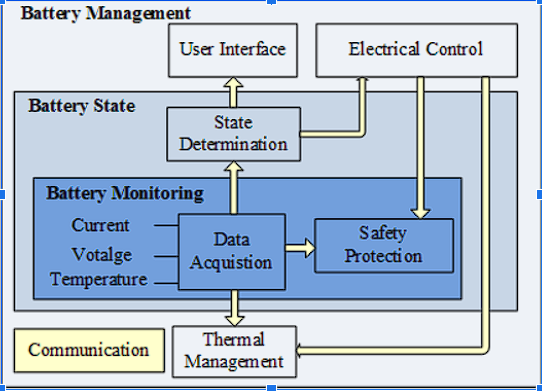
\includegraphics{bms.png}
    \caption{Sự mô tả về một hệ thống quản lý pin }
    \label{fig:enter-label}
\end{figure}

\vspace{7cm}
\subsection{Các phương pháp tối ưu và mô hình fog computing}
Như đã nói ở phần trước, thì sau khi đã đặc tả một số tính chất của hệ thống giám sát pin xe điện gồm: trạng thái sạc - SOC, trạng thái sức khỏe - SOH, vv… Cho nên phần sau đây sẽ mô tả thiết mở rộng với mô hình fog- computing và đưa ra một số phương án tối ưu cho các bài toán ở trên. 
\vspace{10cm}
\begin{figure}
    \centering
    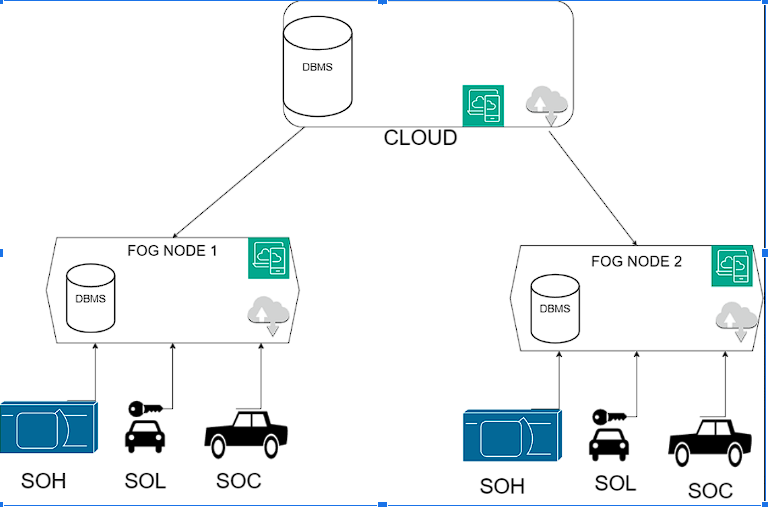
\includegraphics{fog-computing.png}
    \label{fig:enter-label}
\end{figure}
\vspace{5cm}

\textbf{Sử dụng phương pháp chọn khoảng thích hợp để giải quyết bài toán lưu trữ dữ liệu cho State of Charge(SOC) }
\begin{itemize}
    \item[--] Dữ liệu thu thập được về trạng thái sạc: Được biết công thức của State of Charge chứa đại lượng biến thiên theo thời gian t, cho nên nếu phải lưu trữ toàn bộ dữ liệu sẽ làm tốn bộ nhớ lưu trữ và quá trình truy xuất cũng trở nên chậm chạp hơn. 

    Cho nên thay vì ta phải lưu trữ toàn bộ dữ liệu bắn về liên tục (real-time), thì luận văn này đề xuất phương án lưu theo khoảng delta và ngưỡng chọn e, sao cho delta không vượt quá e, thì ta sẽ nhóm lại thành một cụm dữ liệu (cluster) để tối ưu việc lưu trữ.
    
\end{itemize}

\textbf{Sử dụng các mô hình học máy cho các bài toán về state of health và state of life}
\begin{itemize}
    \item [--] Support Vector Machine (SVM)(based model)
Máy vector hỗ trợ (Support Vector Machine - SVM) there một kỹ thuật tính toán mềm phổ biến và được sử dụng rộng rãi trong nhiều lĩnh vực. Nguyên tắc cơ bản của SVM là sử dụng ánh xạ phi tuyến cho việc ánh xạ dữ liệu trong một số lĩnh vực và áp dụng thuật toán tuyến tính trong không gian hàm.
    \item[--] Linear Regression (LR):
Các thuật toán hồi quy tuyến tính sẽ được áp dụng nếu đầu ra là một biến liên tục. Ngược lại, các thuật toán phân loại được áp dụng khi đầu ra được chia thành các phần như đạt/không đạt, tốt/trung bình/kém, vv. Chúng ta có các thuật toán hồi quy khác nhau hoặc phân loại hành vi, trong đó thuật toán hồi quy tuyến tính (Linear Regression - LR) là thuật toán hồi quy cơ bản. 
    \item[--] Ensemble Bagging (EBa):
Bagging (Bootstrap Aggregating) there một meta-algorithm trong học máy được thiết kế để tăng cường độ chính xác và độ chính xác của các thuật toán học máy trong phân loại thống kê và hồi quy. Nó cũng giảm phương sai và giúp tránh hiện tượng quá khớp. Bagging là một cách để giảm bớt sự không chắc chắn của ước lượng bằng cách tạo ra các dữ liệu bổ sung cho việc kiểm tra tập dữ liệu bằng cách tạo ra các biến thể sao chép để tạo ra các tập dữ liệu ban đầu khác nhau . Boosting là một chiến lược lặp lại dựa trên mô tả trước đó để điều chỉnh trọng số của quan sát.

 
\end{itemize}

\section{KẾ HOẠCH TRIỂN KHAI}
Trong thời gian sắp tới của luận văn, tôi dự định triển khai các công việc như sau:\\
- Chuẩn bị dữ liệu, chuẩn hóa bao gồm tiền xử lý nếu có\\
- Sử dụng các mô hình học máy để hỗ trợ đánh giá SOH, SOL\\
- Tối ưu lượng thông tin lưu trữ dữ liệu và đẩy lên cloud \\
- Sử dụng các phương pháp và hiện thực mô hình \\
- Kết hợp các mô hình cloud-computing \\
- Tổng hợp kết quả và viết báo cáo\\
- Thời gian thực hiện các công việc ở biểu đồ sau:

\begin{figure}[h]
\begin{center}
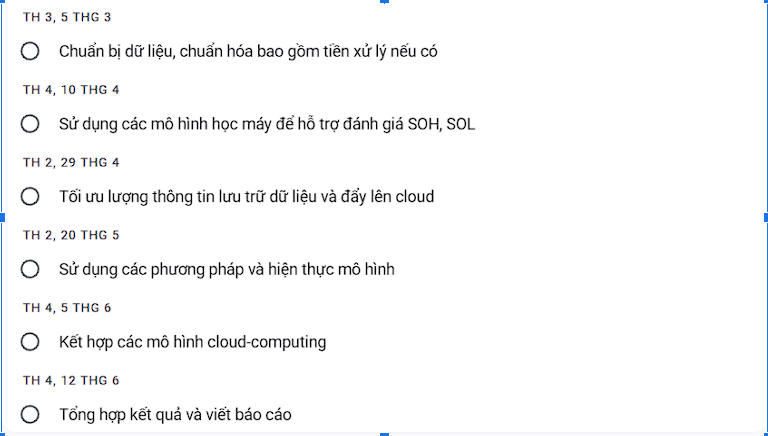
\includegraphics[width=5in]{plan.png}
\end{center}
\end{figure} 

\vspace{5cm}
\section{NỘI DUNG DỰ KIẾN CỦA LUẬN VĂN}

Nội dung báo cáo của luận văn dự kiến sẽ bao gồm các phần như sau:\\

\textbf{Chương 1: Giới thiệu}. Trong chương này sẽ trình bày một số vấn đề cơ bản của đề tài, nêu lên sự quan trọng của việc kiểm tra và giám sát thành phần trong xe điện trong lĩnh vực dữ liệu số hóa. Từ đó thấy được tầm quan trọng của đề tài để xác định rõ phạm vi và đối tượng nghiên cứu, hướng giải quyết của đề tài.
\\

\textbf{Chương 2: Các công trình nghiên cứu liên quan.} Trong chương này sẽ trình bày các công trình nghiên cứu liên quan. Tìm hiểu các phương pháp giải quyết vấn đề cũng như phạm vi, giới hạn của các nghiên cứu đó. Từ đó đánh giá tính khả thi của đề tài.\\

\textbf{Chương 3: Hiện thực và thử nghiệm mô hình. } Trong chương này sẽ trình bày chi tiết cách thức hiện thực của mô hình. Bao gồm các bước xây dựng và huấn luyện mô hình, sử dụng các mô hình và heuristic để giải quyết bài toán.\\

\textbf{Chương 4: Kết quả và đánh giá.} Trong chương này sẽ nêu ra các kết quả đạt được của mô hình, cũng như phương pháp đánh giá các kết quả đó.\\

\textbf{Chương 5: Kết luận.} Trong chương này sẽ tóm lại các ưu điểm và nhược điểm của mô hình và đưa ra các hướng nghiên cứu phát triển hệ thống trong tương lai.\\

\section{KẾT LUẬN}
Việc giám sát và quản lý pin đóng vai trò quan trọng trong đảm bảo hiệu suất, tuổi thọ và an toàn của hệ thống pin trên xe điện. Các công trình nghiên cứu liên quan đã tập trung vào các khía cạnh quan trọng như ước lượng trạng thái sạc và sức khỏe pin, chẩn đoán và tiên đoán lỗi, và quản lý thông minh của pin.\\

Để giám sát pin trên xe điện một cách hiệu quả, cần phải có hệ thống quản lý pin (BMS) thông minh và chính xác. BMS sẽ thu thập dữ liệu về trạng thái pin như trạng thái sạc, nhiệt độ, điện áp và dòng điện, sau đó phân tích và đưa ra các quyết định để bảo vệ pin và tối ưu hóa hiệu suất sử dụng năng lượng.\\

Công nghệ và phương pháp giám sát pin ngày càng phát triển, bao gồm sự kết hợp của cảm biến, hệ thống ghi dữ liệu, trí tuệ nhân tạo và học máy. Các phương pháp này giúp ước lượng trạng thái sạc và sức khỏe pin một cách chính xác, phát hiện và chẩn đoán lỗi một cách nhanh chóng, và dự đoán tuổi thọ còn lại của pin.\\

Thông qua việc nghiên cứu và áp dụng các công trình liên quan, có thể nâng cao hiệu suất và tuổi thọ của pin trên xe điện, giúp tăng khả năng di chuyển và đáp ứng nhu cầu của người sử dụng. Đồng thời, việc giám sát pin cũng đóng vai trò quan trọng trong việc đảm bảo an toàn và hạn chế các vấn đề liên quan đến pin như quá nhiệt, quá điện áp hoặc quá dòng điện.\\

Tổng quan, đề tài "Giám sát pin trên xe điện" là một lĩnh vực nghiên cứu quan trọng và đầy triển vọng, đóng góp vào sự phát triển của công nghệ pin và xe điện hiệu quả và bền vững.\\

%\include{bibliography}
\begin{thebibliography}{19}

\bibitem{H. Truong:Rahman:Shenoy:2018} 
H. Truong, S. Rahman, và P. S. Shenoy (2018),
Battery Management Systems in Electric and Hybrid Vehicles.

\bibitem{Benmouiza}
A. Benmouiza và A. Chandra,
State of Charge Estimation of Lithium-Ion Batteries in Electric Vehicles: A Review

\bibitem{Y. Hu}
Y. Hu, L. Wang, và H. Gao,
Real-Time State of Health Estimation for Lithium-Ion Batteries in Electric Vehicles

\bibitem{Y. Li}
Y. Li và C. Mi.,
Data-Driven Fault Diagnosis and Prognosis of Lithium-Ion Batteries in Electric Vehicles

\bibitem{X. Hu}
X. Hu, Y. Li, và C. Mi.,
Intelligent Battery Management and Control for Electric Vehicles

\bibitem{Rui Xiong}
Rui Xiong, Kui Zhang,
Design and implementation of a Battery Big Data Platform Through Intelligent Connected Electric Vehicles

\bibitem{Cheng:2011}
Cheng, K.W.E.; Divakar, B.P.; Wu, H.J.; Ding, K.; Ho, H.F,
Battery-Management System (BMS) and SOC development for electrical vehicles,
\textbf{IEEE Trans. Veh. Technol}, 60, 76--88, 2011

\bibitem{Tipping:2000}
Tipping, M.E,
The Relevance Vector Machine. Advances in Neural Information Processing Systems,
\textbf{MIT Press: Cambridge, MA, USA}, 12, 287--289, 2000

\bibitem{Widodo:2011}
Widodo, A.; Shim, M.C.; Caesarendra, W.; Yang, B.-S,
Intelligent prognostics for battery health monitoring based on sample entropy,
\textbf{Expert Syst. Appl}, 38, 11763--11769, 2011

\bibitem{Chao:2011}
Chao, K.H.; Chen, J.W,
State-of-health estimator based on extension theory with a learning mechanism for lead-acid batteries,
\textbf{Expert Syst. Appl}, 38, 15183--15193, 2011

\bibitem{Moo:2009}
Ng, K.S.; Moo, C.S.; Chen, Y.P.; Hsieh, Y.C,
Enhanced coulomb counting method for estimating state-of-charge and state-of-health of lithium-ion batteries,
\textbf{Appl. Energy}, 86, 1506--1511, 2009

\bibitem{}
State of Charge (SOC) Determination,
\textbf{http://www.mpoweruk.com/soc.htm},
232, 2011

\end{thebibliography}
\end{document}